\section{Training Loss}
The training loss is a measure that is used to determine how well a deep learning model fits the training data. The cross entropy loss was used to compute the loss of the transformer and the CodeBERT model. The experiment was conducted on different configurations of the transformer and the CodeBERT model, for varying numbers of epochs.
\\\\
\textbf{Case I: 50 epochs} \\
\textbf{Transformer} \\
The following graphs illustrate the pattern of training loss for transformers with (6, 6) layers of encoder and decoder and (12, 12) layers of encoder and decoder.
\begin{figure}[H]
\centering
  \begin{subfigure}[h]{0.45\textwidth}
    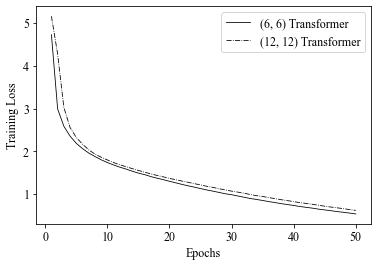
\includegraphics[width=\textwidth]{visualization/ja2pn_50E_6E_6D_vs_12E_12D.png}
    \caption{Java to Python Translation}
    \label{fig:6.1_a}
  \end{subfigure}
  ~
  \begin{subfigure}[h]{0.45\textwidth}
    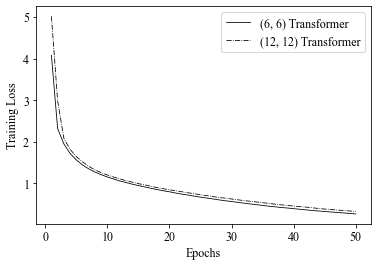
\includegraphics[width=\textwidth]{visualization/pn2ja_50E_6E_6D_vs_12E_12D.png}
    \caption{Python to Java Translation}
    \label{fig:6.1_b}
  \end{subfigure}
\caption[Training loss of the transformer model with 6 encoder layers and 6 decoder layers, and 12 encoder layers and 12 decoder layers, for 50 epochs]{Training loss of the transformer model with 6 encoder layers and 6 decoder layers, and 12 encoder layers and 12 decoder layers, for 50 epochs}
\label{fig:6.1}
\end{figure}
\noindent
The training losses of 0.5366 and 0.6188 were obtained for the transformer model with (6, 6) and (12, 12) layers, respectively, while training the models to translate from Java to Python, as shown in Figure \ref{fig:6.1_a}. In the case of Python to Java translation (Figure \ref{fig:6.1_b}), losses of 0.2692 and 0.3295 were observed for (6, 6) and (12, 12) layers, respectively.
\\\\
\textbf{CodeBERT} \\
The training losses of the models initialized with (6, 6) and (12, 12) layers of CodeBERT are shown in Figure \ref{fig:6.2}.
\begin{figure}[H]
\centering
  \begin{subfigure}[h]{0.45\textwidth}
    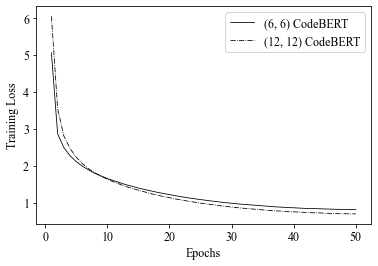
\includegraphics[width=\textwidth]{visualization/codebert_ja2pn_50E_6E_6D_vs_12E_12D.png}
    \caption{Java to Python Translation}
    \label{fig:6.2_a}
  \end{subfigure}
  ~
  \begin{subfigure}[h]{0.45\textwidth}
    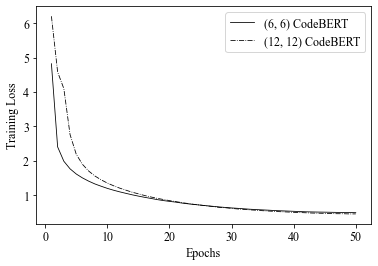
\includegraphics[width=\textwidth]{visualization/codebert_pn2ja_50E_6E_6D_vs_12E_12D.png}
    \caption{Python to Java Translation}
    \label{fig:6.2_b}
  \end{subfigure}
\caption[Training loss of the CodeBERT model with 6 encoder layers and 6 decoder layers, and 12 encoder layers and 12 decoder layers, for 50 epochs]{Training loss of the CodeBERT model with 6 encoder layers and 6 decoder layers, and 12 encoder layers and 12 decoder layers, for 50 epochs}
\label{fig:6.2}
\end{figure}
\noindent
For Java to Python translation, the losses of 0.8076 and 0.6914 were obtained for (6, 6) and (12, 12) layers, respectively; and for Python to Java translation, the losses of 0.4945 and 0.4588 were obtained, respectively.
\\\\
\textbf{Transformer vs CodeBERT} \\
Figure \ref{fig:6.3} shows the transformer and CodeBERT training losses of 0.5366 and 0.8076 for (6, 6) layers and 0.6188 and 0.6914 for (12, 12) layers when trained to translate from Java to Python; and Figure \ref{fig:6.4} shows the losses of 0.2692 and 0.4945 for (6, 6) layers and 0.3295 and 0.4588 for (12, 12) layers of the models when trained to translate from Python to Java.
\begin{figure}[H]
\centering
  \begin{subfigure}[h]{0.45\textwidth}
    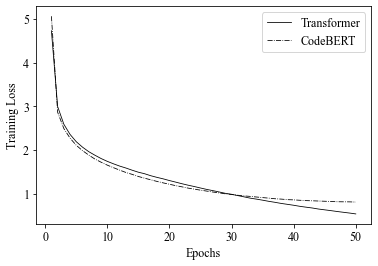
\includegraphics[width=\textwidth]{visualization/transformer_vs_codebert_ja2pn_50E_6E_6D.png}
    \caption{Training loss of the models with 6 encoder layers and 6 decoder layers}
    \label{fig:6.3_a}
  \end{subfigure}
  ~
  \begin{subfigure}[h]{0.45\textwidth}
    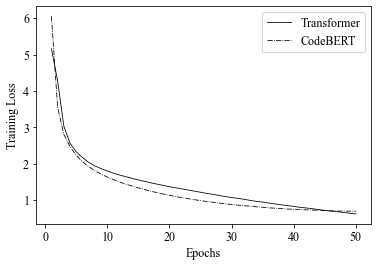
\includegraphics[width=\textwidth]{visualization/transformer_vs_codebert_ja2pn_50E_12E_12D.png}
    \caption{Training loss of the models with 12 encoder layers and 12 decoder layers}
    \label{fig:6.3_b}
  \end{subfigure}
\caption[Training loss of the transformer and CodeBERT model in Java to Python translation for 50 epochs]{Training loss of the transformer and CodeBERT model in Java to Python translation for 50 epochs}
\label{fig:6.3}
\end{figure}

\begin{figure}[H]
\centering
  \begin{subfigure}[h]{0.45\textwidth}
    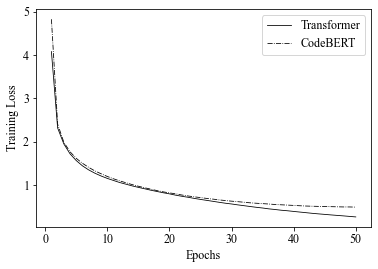
\includegraphics[width=\textwidth]{visualization/transformer_vs_codebert_pn2ja_50E_6E_6D.png}
    \caption{Training loss of the models with 6 encoder layers and 6 decoder layers}
    \label{fig:6.4_a}
  \end{subfigure}
  ~
  \begin{subfigure}[h]{0.45\textwidth}
    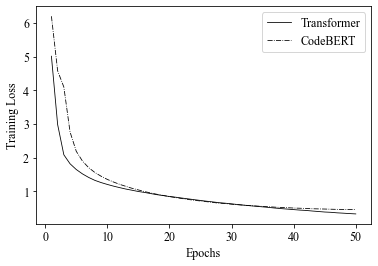
\includegraphics[width=\textwidth]{visualization/transformer_vs_codebert_pn2ja_50E_12E_12D.png}
    \caption{Training loss of the models with 12 encoder layers and 12 decoder layers}
    \label{fig:6.4_b}
  \end{subfigure}
\caption[Training loss of the transformer and CodeBERT model in Python to Java translation for 50 epochs]{Training loss of the transformer and CodeBERT model in Python to Java translation for 50 epochs}
\label{fig:6.4}
\end{figure}
\medskip
\smallskip
\textbf{Case II: 100 epochs} \\
\textbf{Transformer} \\
Figure \ref{fig:6.5_a} depicts the training loss for (6, 6) and (12, 12) transformers while training from Java to Python; the final losses are 0.1176 and 0.1461, respectively. Similarly, Figure \ref{fig:6.5_b} shows the losses of 0.0515 and 0.0697 observed in models while training in the Python to Java direction. 
\begin{figure}[H]
\centering
  \begin{subfigure}[h]{0.45\textwidth}
    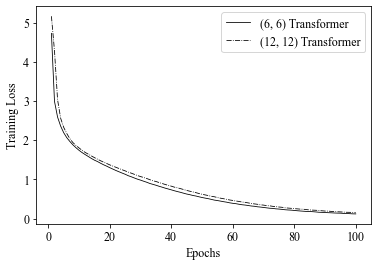
\includegraphics[width=\textwidth]{visualization/ja2pn_100E_6E_6D_vs_12E_12D.png}
    \caption{Java to Python Translation}
    \label{fig:6.5_a}
  \end{subfigure}
  ~
  \begin{subfigure}[h]{0.45\textwidth}
    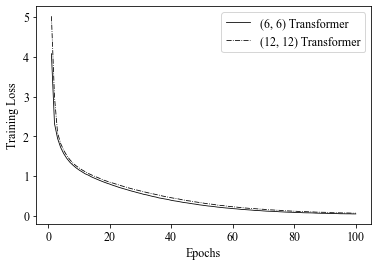
\includegraphics[width=\textwidth]{visualization/pn2ja_100E_6E_6D_vs_12E_12D.png}
    \caption{Python to Java Translation}
    \label{fig:6.5_b}
  \end{subfigure}
\caption[Training loss of the transformer model with 6 encoder layers and 6 decoder layers, and 12 encoder layers and 12 decoder layers, for 100 epochs]{Training loss of the transformer model with 6 encoder layers and 6 decoder layers, and 12 encoder layers and 12 decoder layers, for 100 epochs}
\label{fig:6.5}
\end{figure}
\medskip
\smallskip
\textbf{CodeBERT} \\
Figure \ref{fig:6.6} shows the loss for (6, 6) and (12, 12) CodeBERT models trained in Java to Python direction; the losses are 0.3088 and 0.5233, respectively. In Java to Python direction, the losses observed are 0.1381 and 0.1575, respectively.
\begin{figure}[H]
\centering
  \begin{subfigure}[h]{0.45\textwidth}
    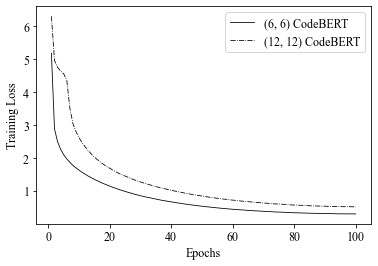
\includegraphics[width=\textwidth]{visualization/codebert_ja2pn_100E_6E_6D_vs_12E_12D.png}
    \caption{Java to Python Translation}
    \label{fig:6.6_a}
  \end{subfigure}
  ~
  \begin{subfigure}[h]{0.45\textwidth}
    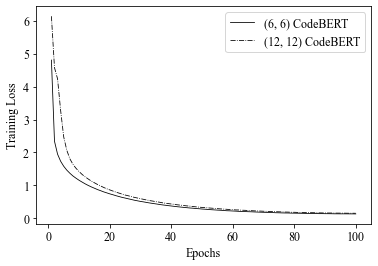
\includegraphics[width=\textwidth]{visualization/codebert_pn2ja_100E_6E_6D_vs_12E_12D.png}
    \caption{Python to Java Translation}
    \label{fig:6.6_b}
  \end{subfigure}
\caption[Training loss of the CodeBERT model with 6 encoder layers and 6 decoder layers, and 12 encoder layers and 12 decoder layers, for 50 epochs]{Training loss of the CodeBERT model with 6 encoder layers and 6 decoder layers, and 12 encoder layers and 12 decoder layers, for 50 epochs}
\label{fig:6.6}
\end{figure}
\medskip
\smallskip
\textbf{Transformer vs CodeBERT}\\
The training losses of (6, 6) and (12, 12) layers transformer and CodeBERT models in Java to Python translation direction are shown in Figure \ref{fig:6.7}. For (6, 6) layers the loss at the end of epoch for the transformer model is 0.1176 and for the CodeBERT model is 0.3088. For (12, 12) layers the loss for the tranformer model is 0.1461 and the CodeBERT model is 0.5233.
\begin{figure}[H]
\centering
  \begin{subfigure}[h]{0.45\textwidth}
    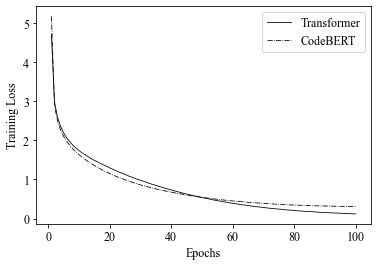
\includegraphics[width=\textwidth]{visualization/transformer_vs_codebert_ja2pn_100E_6E_6D.png}
    \caption{Training loss of the models with 6 encoder layers and 6 decoder layers}
    \label{fig:6.7_a}
  \end{subfigure}
  ~
  \begin{subfigure}[h]{0.45\textwidth}
    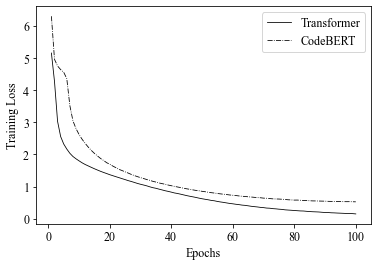
\includegraphics[width=\textwidth]{visualization/transformer_vs_codebert_ja2pn_100E_12E_12D.png}
    \caption{Training loss of the models with 12 encoder layers and 12 decoder layers}
    \label{fig:6.7_b}
  \end{subfigure}
\caption[Training loss of the transformer and CodeBERT model in Java to Python translation for 100 epochs]{Training loss of the transformer and CodeBERT model in Java to Python translation for 100 epochs}
\label{fig:6.7}
\end{figure}
Similarly, the training losses for the transformer and CodeBERT models in Python to Java translation direction are show in Figure \ref{fig:6.8}. The transformer and CodeBERT model with (6, 6) layers have training loss 0.0514, 0.1381 respectively, and with (12, 12) layers have 0.0697, 0.1575, respectively.
\begin{figure}[H]
\centering
  \begin{subfigure}[h]{0.45\textwidth}
    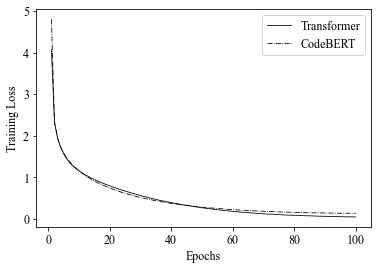
\includegraphics[width=\textwidth]{visualization/transformer_vs_codebert_pn2ja_100E_6E_6D.png}
    \caption{Training loss of the models with 6 encoder layers and 6 decoder layers}
    \label{fig:6.8_a}
  \end{subfigure}
  ~
  \begin{subfigure}[h]{0.45\textwidth}
    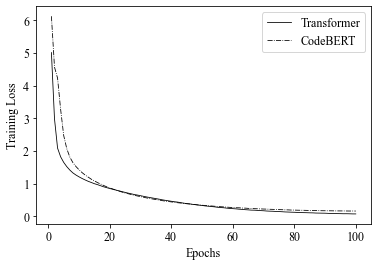
\includegraphics[width=\textwidth]{visualization/transformer_vs_codebert_pn2ja_100E_12E_12D.png}
    \caption{Training loss of the models with 12 encoder layers and 12 decoder layers}
    \label{fig:6.8_b}
  \end{subfigure}
\caption[Training loss of the transformer and CodeBERT model in Python to Java translation for 100 epochs]{Training loss of the transformer and CodeBERT model in Python to Java translation for 100 epochs}
\label{fig:6.8}
\end{figure}
%\vspace*{-32pt}
\section{Results}
The BLEU and CodeBLEU scores of the transformer and CodeBERT models obtained for 627 testing samples are shown in Table \ref{table:6.1} (Java to Python) and Table \ref{table:6.2} (Python to Java).
\begin{table}[H]
\centering
\def\arraystretch{1.25}
\caption{BLEU, CodeBLEU, WNM, SM, and DM scores for Java to Python translation}
\label{table:6.1}
\begin{tabular}{|P{1.15cm}|P{1.15cm}|c|c|c|c|c|c|c|} \hline
\textbf{No. of epochs} & \textbf{No. of layers} & \textbf{Model} & \textbf{BLEU} & \textbf{CodeBLEU} & \textbf{WNM} & \textbf{SM} & \textbf{DM}\\ \hline
\multirow{4}{*}{50} & \multirow{2}{*}{6} & Transformer & \textbf{0.2812} & \textbf{0.2802} & \textbf{0.2828} & 0.3137 & 0.2430 \\ \cline{3-8}
			      & 			      & CodeBERT & 0.1294 & 0.2109 & 0.1321 & \textbf{0.3491} & 0.2334 \\ \cline{2-8}
 			      & \multirow{2}{*}{12} & Transformer & 0.2627 & 0.2724 & 0.2642 & 0.3227 & 0.2400 \\ \cline{3-8}
			      & 			      & CodeBERT & 0.0977 & 0.1897 & 0.1028 & 0.3439 & 0.2152 \\ \hline
\multirow{4}{*}{100} & \multirow{2}{*}{6} & Transformer & 0.2659 & 0.2733 & 0.2683 & 0.3097 & \textbf{0.2492} \\ \cline{3-8}
			      & 			      & CodeBERT & 0.1512 & 0.2233 & 0.1539 & 0.3485 & 0.2401 \\ \cline{2-8}
 			      & \multirow{2}{*}{12} & Transformer & 0.2519 & 0.2656 & 0.2536 & 0.3154 & 0.2415 \\ \cline{3-8}
			      & 			      & CodeBERT & 0.1067 & 0.1745 & 0.1092 & 0.3063 & 0.1760 \\ \hline
\end{tabular}
\end{table}

\begin{table}[H]
\centering
\def\arraystretch{1.25}
\caption{BLEU, CodeBLEU, WNM, SM, and DM scores for Python to Java translation}
\label{table:6.2}
\begin{tabular}{|P{1.15cm}|P{1.15cm}|c|c|c|c|c|c|c|} \hline
\textbf{No. of epochs} & \textbf{No. of layers} & \textbf{Model} & \textbf{BLEU} & \textbf{CodeBLEU} & \textbf{WNM} & \textbf{SM} & \textbf{DM}\\ \hline
\multirow{4}{*}{50} & \multirow{2}{*}{6} & Transformer & 0.3883 & 0.4016 & 0.3990 & 0.4715 & 0.3434 \\ \cline{3-8}
			      & 			      & CodeBERT & 0.2747 & 0.3495 & 0.3006 & 0.4857 & 0.3234 \\ \cline{2-8}
 			      & \multirow{2}{*}{12} & Transformer & 0.3633 & 0.3841 & 0.3744 & 0.4591 & 0.3358 \\ \cline{3-8}
			      & 			      & CodeBERT & 0.2580 & 0.3299 & 0.2770 & 0.4644 & 0.3112 \\ \hline
\multirow{4}{*}{100} & \multirow{2}{*}{6} & Transformer & \textbf{0.3891} & \textbf{0.4018} & \textbf{0.4012} & 0.4613 & \textbf{0.3526} \\ \cline{3-8}
			      & 			      & CodeBERT & 0.2938 & 0.3727 & 0.3203 & \textbf{0.5172} & 0.3458 \\ \cline{2-8}
 			      & \multirow{2}{*}{12} & Transformer & 0.3652 & 0.3837 & 0.3778 & 0.4461 & 0.3434 \\ \cline{3-8}
			      & 			      & CodeBERT & 0.2936 & 0.3697 & 0.3183 & 0.5120 & 0.3424 \\ \hline
\end{tabular}
\end{table}

\section{Analysis}
In order to choose the appropriate model for program translation, the study evaluates the BLEU and CodeBLEU scores of the CodeBERT and the transformer models. The study uses trained models to translate programs from the test dataset and compute BLEU and CodeBLEU scores. It determines whether the Python to Java program translation models have equivalent BLEU and CodeBLEU scores to the Java to Python program translation models.
\\\\
The transformer model with 6 layers has a lower training loss than the model with 12 layers over a period of 50 epochs. Both the 6-layer Java to Python transformer translation model and the 6-layer Python to Java transformer translation model have losses of 0.5366 and 0.2692, respectively. In the case of the CodeBERT models trained for 50 epochs, the 12-layer models exhibit less loss than the 6-layer models. The loss for the 12-layer Java to Python CodeBERT model is 0.6914, and the loss for the Python to Java CodeBERT model is 0.4588. In comparison to CodeBERT models with 6 layers, transformer models with 6 layers produce lower training loss. The 6-layer transformer model has a loss of 0.5366 and 0.2692 when training from Java to Python and Python to Java, respectively. The 12-layer transformer also performs better than the 12-layer CodeBERT in terms of training loss, with losses of 0.3295 and 0.6188 when training from Python to Java and Java to Python, respectively. Even for 100 epochs, the 6-layer transformer models have less training loss than the 12-layer transformer models. Likewise, 6-layer CodeBERT models show less loss than 12-layer CodeBERT models after 100 training epochs. For 100 training epochs, the CodeBERT models also suffer from high training loss in comparison to the transformer models.
\\\\
The results shown in Table 6.1 demonstrate that the transformer model with 6 encoder and 6 decoder layers, trained for 50 epochs to translate from Java to Python, received the highest BLEU and CodeBLEU scores, with values of 0.2812 and 0.2802, respectively. According to the results shown in Table 6.2, the transformer model, trained for 100 epochs to translate from Python to Java, achieved the highest BLEU and CodeBLEU scores, respectively, of 0.3891 and 0.4018. This model also has 6 encoder and 6 decoder layers. Additionally, the results demonstrate that Python to Java translation models have higher BLEU and CodeBLEU scores than Java to Python translation models.
\\\\
In this study, the transformer models have performed better than the CodeBERT models in terms of BLEU and CodeBLEU scores. In addition to this, the transformer models have achieved higher WNM, and DM scores than the CodeBERT models. However, the SM scores of the transformer models are lower than those of the CodeBERT models.





